A point $P$ is chosen in the interior of $\triangle ABC$ so that when lines are drawn through $P$ parallel to the sides of $\triangle ABC$, the resulting smaller triangles, $t_1$, $t_2$, and $t_3$ in the figure, have areas 4, 9, and 49, respectively. Find the area of $\triangle ABC$.
\begin{center}
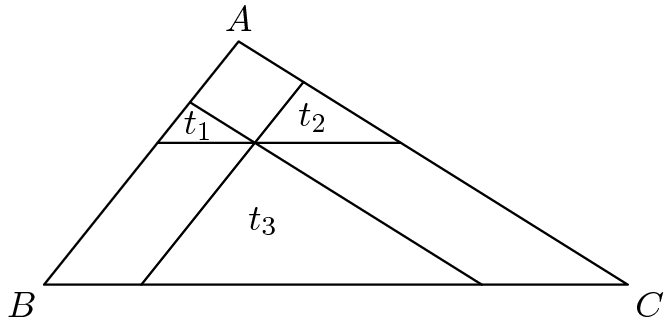
\includegraphics[width = 67.0mm]{img/fig0.png}
\end{center}